\documentclass[10pt]{datasheet}
\usepackage[utf8]{inputenc}
\usepackage[english]{babel}
\usepackage[english]{isodate}
\usepackage{graphicx}
\graphicspath{ {./images/} }
\usepackage{pgfplots}
\usepackage{circuitikz}
\usetikzlibrary{calc}
\title{Flower Power System}
\author{RathjeVT}
\date{December 2023}
\companylogo{\Huge $\nabla$ RathjeVT}

\begin{document}
\maketitle

\section{Features}

\begin{itemize}
\item{Centrallized DMX control of many different devices}
\item{Custom components can be built}
\item{Simple installation}
\item{Fast module switching times due to universal plug system}
\end{itemize}

\section{Modules}

\begin{itemize}
\item{RVT PSU 12V}
\item{RVT Flower Power}
\item{RVT Flower Station 1}
\item{RVT Flower Station 2}
\item{RVT Flower Spots}
\end{itemize}

\section{General Description}
The Flower Power System is a unique light control system designed to provide an universal
way to control custom lightning modules via DMX-512. It is very easy to design new modules for 
the system. Therefore, this system can be used in future too.

\vfill\break

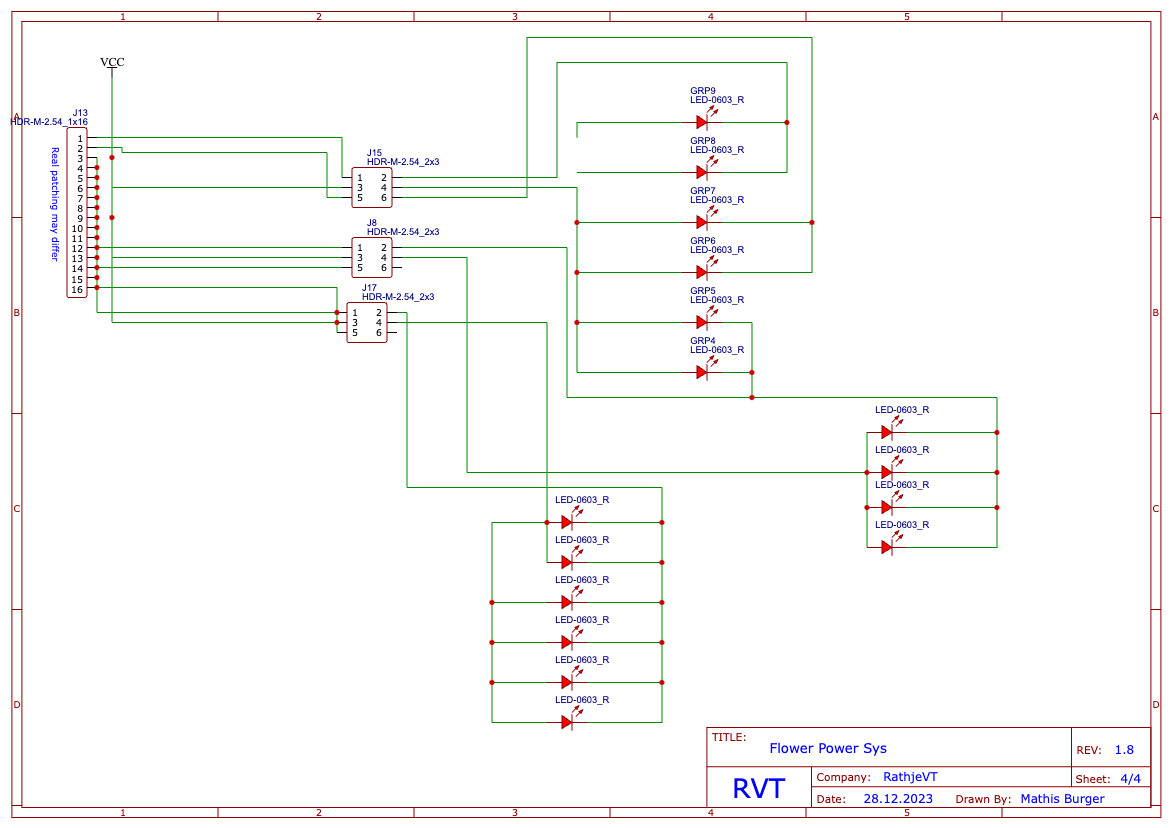
\includegraphics[scale=0.2]{Flower Power System.png}
\onecolumn

% Next Page

\section{Electrical Specifications}
All specifications are in $-10\degree C \leq T_A \leq 60\degree C$ unless otherwise noted.

\begin{table}[h]
\begin{threeparttable}
\caption{Internal specifications}
\begin{tabularx}{\textwidth}{l | c | c}
    \thickhline
    \textbf{Module} & \textbf{Working Voltage} & \textbf{Notes} \\
    \hline
    RVT PSU  & 230V\tnote{1} / 12V & Provides the system with power.  \\
    RVT Flower Power & 12V & Processes the DMX input and triggers deterministically. \\
    RVT Flower Station 1 & 12V & Has 3 seperate groups for controlling light.  \\
    RVT Flower Station 1 & 12V & Has 1 group for controlling light.  \\
    \hline
    \thickhline
\end{tabularx}
\begin{tablenotes}
\item[1]{Touching high voltage components may lead to electrical destruction of the human body. Please first unplug the system of the wall before you work on it.}
\end{tablenotes}
\end{threeparttable}
\end{table}

\section{Electrical module guidelines}

For using the system without any problems you will need to check your whole system for these restrictions:
\begin{itemize}
\item{All modules are able to run on 12V or 24V.}
\item{The system only operates on one specific voltage (12V or 24V).}
\item{The PSU is able to output the exact voltage that is required by the system configuration.}
\item{The total current should not be about the maximum specifications of the thinnest cable in the system.}
\item{All system modules should have an deterministic current flow.}
\item{Connecting modules in series is not allowed}
\end{itemize}

Before installation, the modules should be tested seperated of the system within a demo system or with a simple PSU.
Plugging corrupted modules into a functional system can lead to misfunctions and may also destroy important controller circuits.

\section{Module testing}

If you test the modules following criterias should match the new module:
\begin{itemize}
\item{The rated voltage of all components is the same.}
\item{The module can operate at least 12 hours without failure.}
\item{The maximum current at load is below the maximum current of the thinnest used cable in the \textbf{system}.}
\end{itemize}

\textbf{Note:} Another module check should be performed by a person who is good at EI or ECS.


\pagebreak

\section{Flower Power System wiring}

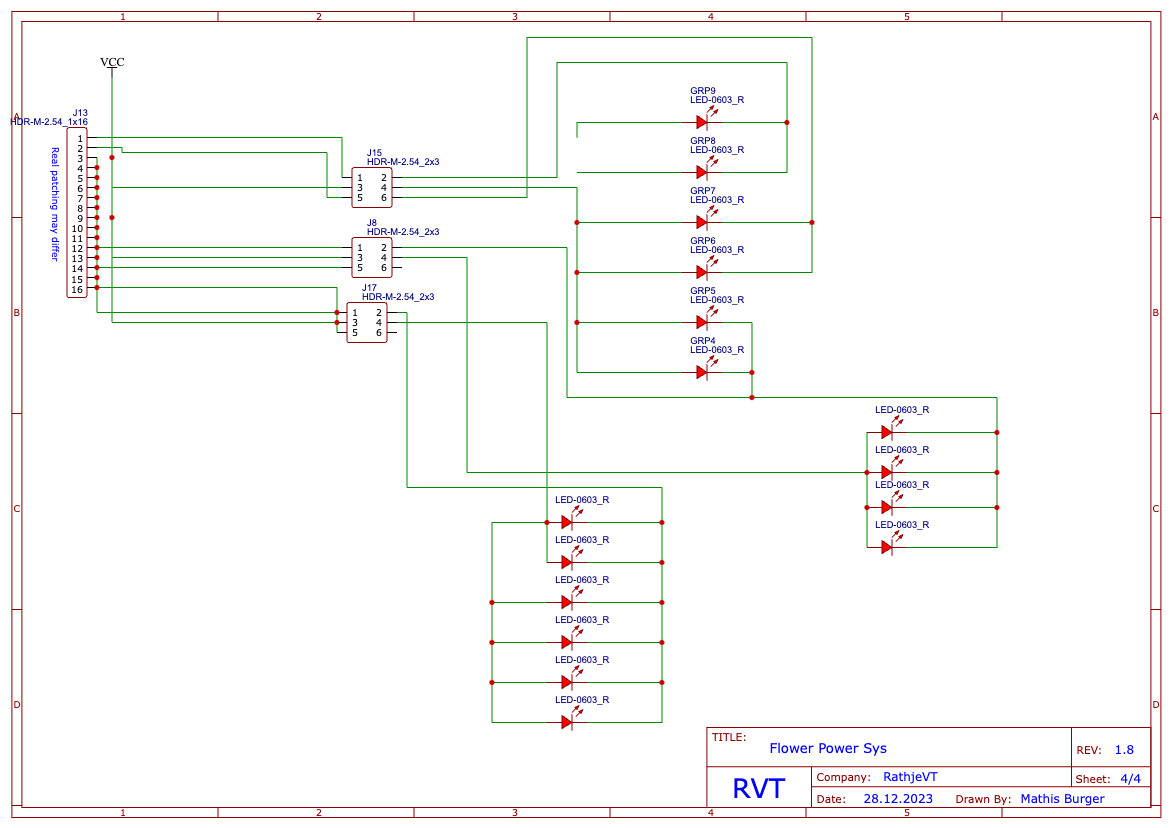
\includegraphics[scale=0.4]{Flower Power System.png}

\textbf{Note:} The wiring of the DMX-512 decoder may differ to the installed due to simplification in DMX address patching.

\section{Extending the system}

It is possible to extend the system by plugging some cables in the leftover ports of the DMX-512 decoder. You will have to use 12V rated hardware. Otherwise your hardware
will be broken or the system will not output enough power to serve your device. Therefore, only 12V hardware can be used with this system. 
The Flower Power controller itself supports up to 24V. For 24V support you will need to have an 24V PSU alongside with only 24V lightning hardware.

\pagebreak

\section{Flower Power}

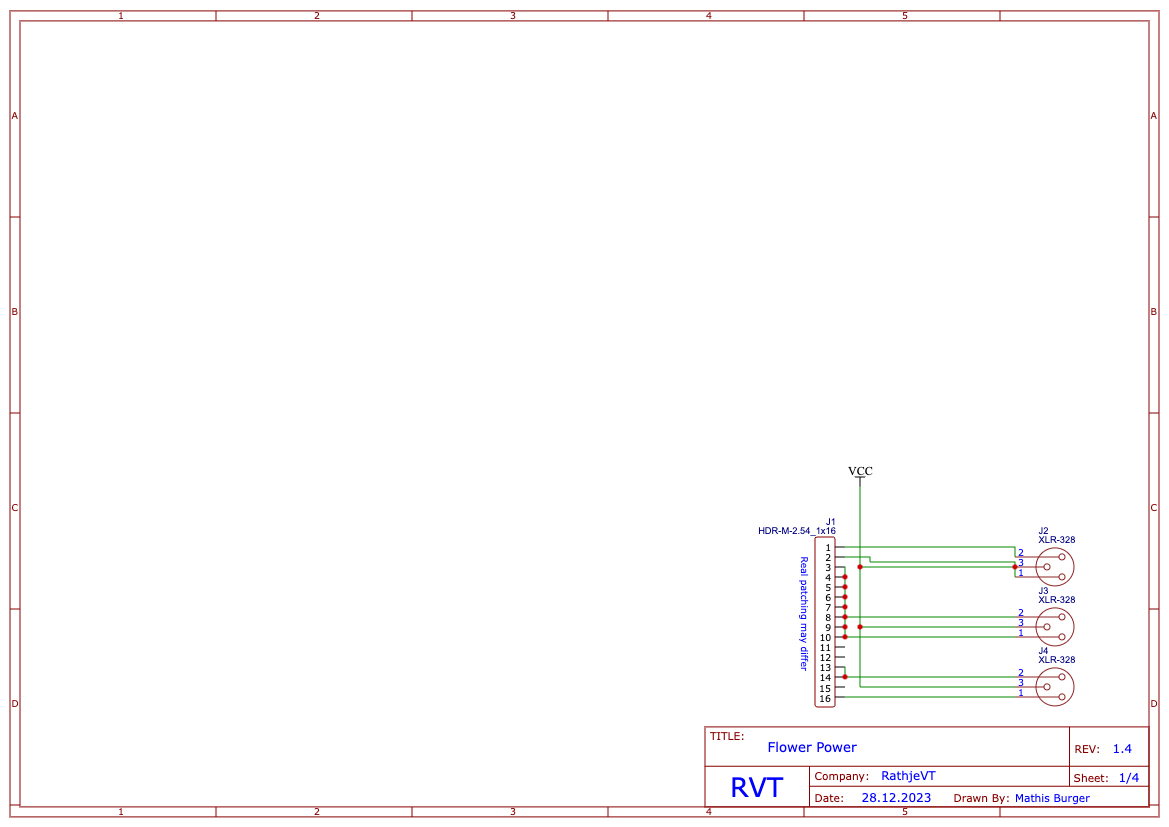
\includegraphics[scale=0.4]{Flower Power.png}

The Flower power is the core controller of the system. It consumes 12V input voltage from the PSU and decides deterministically which GND should be unlocked for current.
The DMX start address can be programmed by a 9-Bit dual in-line package switch. The 10th switch of the DIP is used for a demo mode. It can be used to test the device without a DMX source.
It should be disabled for the use with DMX-512 to work properly. 

\section{Module connection}

Currently, six pins are used for MMC (Mobile Module Connect). These can be used for all modules that support MMC patching.
The MMC patching can be extracted from the Flower Station E-patching plans. The other unused L<n> pins are just switchable GND current flow ports.
The maximum rate voltage for MMC is 24V. If you want to use higher voltages you will have to use another system. The L<n> ports can be used with 12V or 24V.

\pagebreak

\section{Flower Station 1}

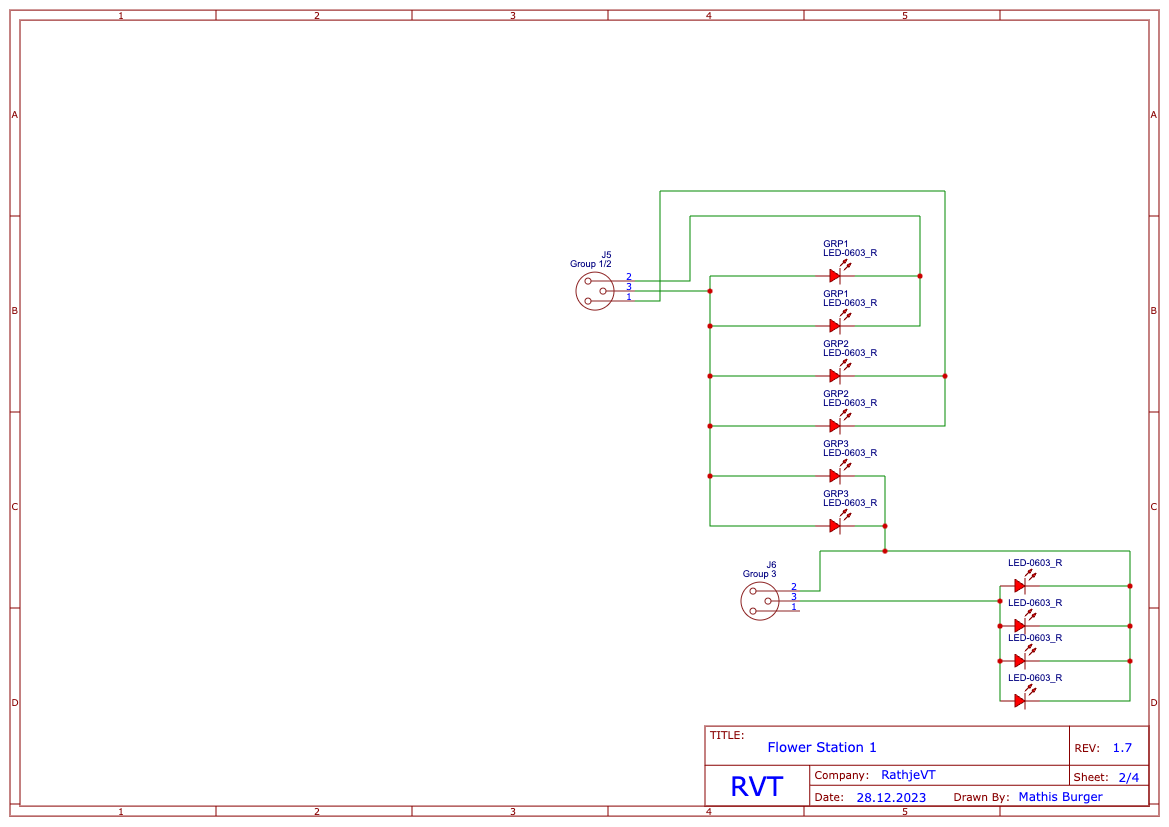
\includegraphics[scale=0.4]{Flower Station 1.png}

The Flower Station 1 is the highest tier station. It supports up to 3 parallel groups with two MMC ports. It is designed to be moved freely.
The big flower technically has three groups, but the first group is directly connected to the side flower group. Therefore there are only two groups
that are exclusively for the big flower. This also means there is no way to only use the side flowers without the big flower. One of the groups is always enabled
when the side flowers are enabled.

\section{Electrical specifications}
\begin{table}[h]
\begin{threeparttable}
\begin{tabularx}{\textwidth}{l | c | c | c | c}
    \thickhline
    \textbf{Group} & \textbf{Voltage (V)} & \textbf{Resistor (\ohm)} & \textbf{Current (A)} & \textbf{Controls} \\
    \hline
    Group 1  & 12V & 1k\ohm & 0.25A & Inner big and side flowers\\
    Group 2  & 12V & 5k\ohm & 0.5A & LED-strip of big flower\\
    Group 3  & 12V & 1k\ohm & 0.25A & Inner big flower \\
    \hline
    \thickhline
\end{tabularx}
\begin{tablenotes}
\end{tablenotes}
\end{threeparttable}
\end{table}

\section{Flower Station 2}

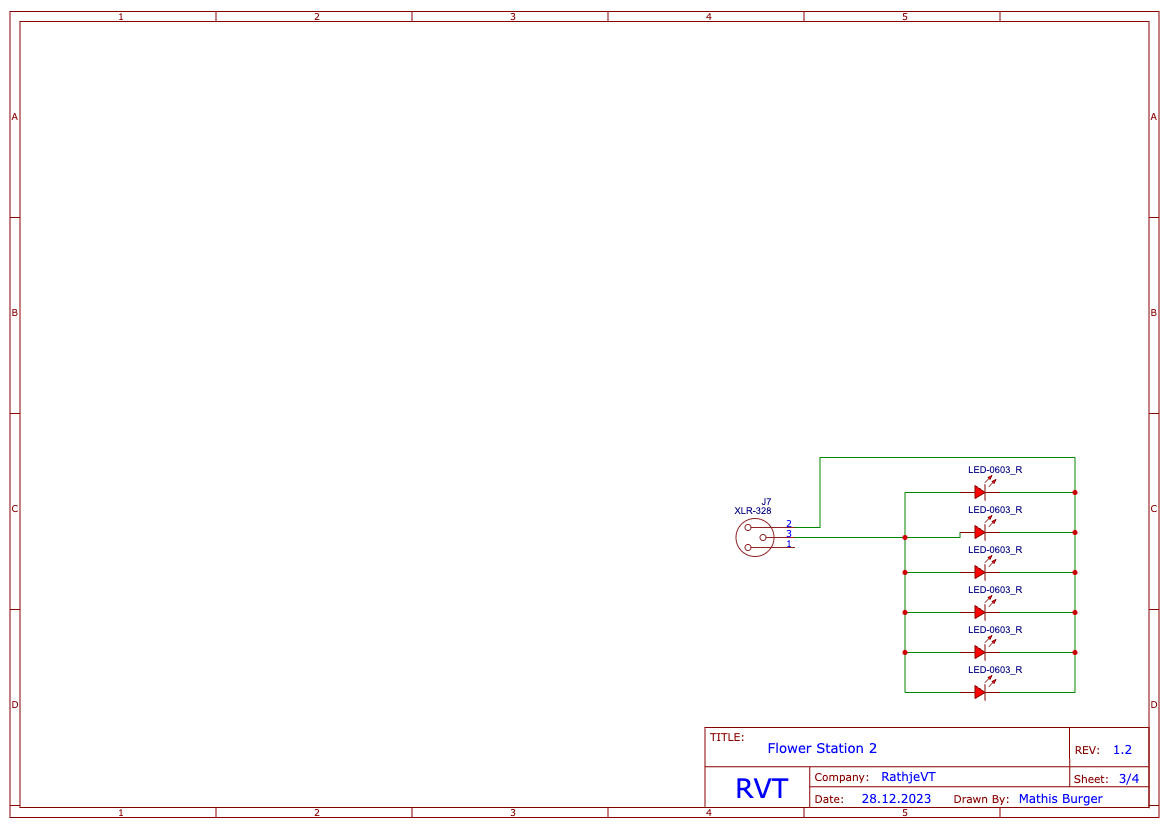
\includegraphics[scale=0.4]{Flower Station 2.png}

The Flower Station 2 is the default station that only has one group to control the flowers. MMC would support another group. So if needed, another group could be integrated. 
The station is only rated for 12V. The soldering is fixed at the MMC port, but can be removed easily. It is important to check the soldering of this station regularly to make sure it functions
properly without the risk of failture during use. Fixing soldering would take at least one hour which is not the time window available at a critical situation. 

\section{Electrical specifications}
\begin{table}[h]
\begin{threeparttable}
\begin{tabularx}{\textwidth}{l | c | c | c | c}
    \thickhline
    \textbf{Group} & \textbf{Voltage (V)} & \textbf{Resistor (\ohm)} & \textbf{Current (A)} & \textbf{Controls} \\
    \hline
    Group 1  & 12V & 1k\ohm & 0.25A & Inner big and side flowers\\
    \hline
    \thickhline
\end{tabularx}
\begin{tablenotes}
\end{tablenotes}
\end{threeparttable}
\end{table}

\textbf{Note:} This station has only one MMC port but one leftover group. This group can be used to control the flowers seperatly if the
station is modified. This could bring more differntiation and complexity. 

\pagebreak

\section{Legal and further information}

The Flower Power System is property of RathjeVT and can only be used by people who got the agreement of usage. 
This sheet may not provide the newest concepts of the system. Therefore, the e-patching may differ to your installation.
It is only for the understanding of the system and not ment for bugfixing. 

Furthermore, there are no electrical calculations provided that are required to operate the system safely with new modules. These calculations
should be done by an expert who knows what he does. 

RathjeVT does not take warranty for misfunctional systems, because it is easy to break if not installed or operated correctly. So make sure before
you start using the system you are informed well enough about the functionality and e-tech basics that are required to fully understand the system.
DMX-512 misusage that leads to system failure is not a system problem, but a light operator problem.

\end{document}